\begin{exo}
	Sur les $170$ couverts servis dans un restaurant un midi, $100$ clients ont pris une entrée et un plat, $110$ ont pris un plat et un dessert.

	Parmi ceux-ci, $80$ ont pris l'entrée, le plat et le dessert. Certains aussi n'ont pris qu'un plat sans entrée ni dessert.

	On choisit au hasard une personne qui a déjeuné dans ce restaurant et on considère les événements :
	\begin{itemize}
		\item $A$ : \og{} le client a pris une entrée \fg{}
		\item $B$ : \og{} le client a pris un dessert \fg{}
	\end{itemize}

	\begin{enumerate}
		\item Déterminer $P(A)$ et $P(B)$.
		\item Reproduire et compléter le diagramme ci-dessous.
	\end{enumerate}
	\begin{center}
		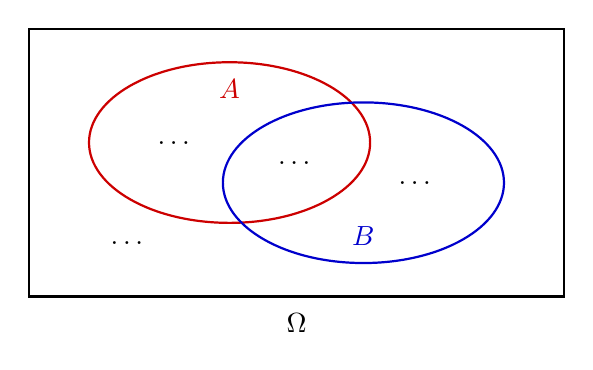
\begin{tikzpicture}[scale=0.85]
			\draw[thick] (0,0) rectangle (8,4);
			\node at (4,-0.4) {$\Omega$};

			\draw[red!80!black, thick] (3,2.3) ellipse (2.1 and 1.2);
			\node[red!80!black] at (3,3.1) {$A$};
			\node at (2.2,2.3) {\dots};

			\draw[blue!80!black, thick] (5,1.7) ellipse (2.1 and 1.2);
			\node[blue!80!black] at (5,0.9) {$B$};
			\node at (5.8,1.7) {\dots};

			\node at (4,2) {\dots};
			\node at (1.5,0.8) {\dots};
		\end{tikzpicture}
	\end{center}
	\begin{enumerate}[resume]
		\item À l'aide du diagramme, déterminer la probabilité qu'un client ait pris un plat seul.
		\item Définir par une phrase l'événement $A \cap B$ et déterminer sa probabilité.
		\item Définir par une phrase l'événement $A \cup B$ et déterminer sa probabilité.
	\end{enumerate}
\end{exo}
